\label{sec:data}

In this section the data which was collected for and in the scope of this thesis is presented, as well as some general information about that.
The dataset is a collection of \acp{ECD}, with \acp{ECC} in German notation.
Seven different \acp{ECC} with connections on two sides were chosen for the scope of this thesis and are shown in figure \ref{fig:used_eccs}.
The number of classes was constrained in order to allow dataset contributors to chose from a small set of symbols.
Under the assumption that each contributer draws the same amount of \acp{ECC} per \ac{ECD} overall the number of samples per class will be higher than with a big amount of symbols.
Therefore, the individual classes are more representative.
Most of the images were taken with a mobile phone, but some were directly drawn on a digital device such as a tablet.
Overall 31 persons contributed to the dataset, with an average of 7.6 \acp{ECD}, a maximum of 30 \acp{ECD} and a minimum of one \ac{ECD}.
For the train, validation test split, \acp{ECD} of 21 persons are used in the train and validation dataset.
In the test dataset those 21 person do not appear, hence 10 previously unseen persons are used for testing.

The difficulty of the task in this thesis increased gradually and more data was always acquired after the difficulty increased.
At first, only images of \acp{ECD} on a white background without annotations were gathered, when that showed promising results, additionally images of \acp{ECD} without annotation but on checkered background were gathered and finally when annotations were added both images with white and checkered background and annotations were acquired.
The total amount of images is shown in table \ref{tab:data_distribution}.
Evaluation was done with all images.
When an image did not contain annotations, then the evaluation of the annotations for this particular image was skipped.


\begin{table}
\begin{center}
\begin{tabular}{l|l|l|l|l|l|l}

    & \textbf{Images} & \textbf{Background} & \textbf{Annotated}  & \textbf{train ratio} & \textbf{valid ratio} & \textbf{test ratio}\\
    \hline
    & 110 & white & & 74.66\% & 6.69\% & 18.65\% \\
    & 17 & checkered & & 17.64\% & 11.77\% & 70.59\%\\
    & 89 & white & \checkmark & 78.65\% & 11.24\% & 10.11\%\\
    & 21 & checkered & \checkmark & 9.52\% & 19.05\% & 71.43\%\\
    \hline
    \textbf{Total} & 239 & & &45.12\% & 12.19\% & 42.69\%\\

\end{tabular}
\caption{Amount of images of \acp{ECD} used in this thesis shown with their underlying background and whether they are annotated or not. Further, the train / validation / test split of the different image types is shown. While this might seem like a big split for test, the number of bounding boxes included in the test set is way smaller and is shown in table \ref{tab:yolo_classes}. For the test dataset 10 persons were used, which are not present in the train and validation dataset.}
\label{tab:data_distribution}
\end{center}
\end{table}

\subsubsection{Labels: Object Detection and Segmentation}

The pipeline in this thesis requires the object detection network \ac{YOLOv4} and the segmentation network \ac{MUnet}.
Therefore, the data was labeled with bounding boxes for \ac{YOLOv4} and with segmentation masks for the \ac{MUnet}.

In table \ref{tab:yolo_classes} all classes used for object detection are presented.
The classes have a major class which corresponds to the \ac{ECC} and an orientation subclass.
Some major classes like resistors have two orientations (horizontal, vertical), while others have four, like diodes (left, top, right, bottom).
The only exception is the text class, which does not have an orientation, since annotations were enforced to be horizontally aligned.

Bounding boxes were annotated with the labeling tool labelme \cite{labelme} in the yolo format which was presented in section \ref{sec:object_detection}.
To also capture parts of the wire in the prediction the bounding boxes were stretched towards the wire around an object.

The segmentation masks were created in a binary fashion, where the foreground corresponds to the drawn \ac{ECD} and the background to everything else.
The masks were created semi-automatically by applying a Canny Edge Detector \cite{canny_edge} on the image.
The resulting edge mask is dilated five times to close potential holes between the edges of a wire and eroded four times to reduce the thickness of the segmentation mask.
The image processing steps become instable once gridded paper is being used, thus each mask is additionally manually fine-tuned, with a simple drawing tool build with the Python version of OpenCV \cite{opencv}.

An example for the \ac{YOLO} bounding boxes and the segmentation mask labels can be found in figure \ref{fig:example_labels}.

\begin{figure}
\begin{center}

    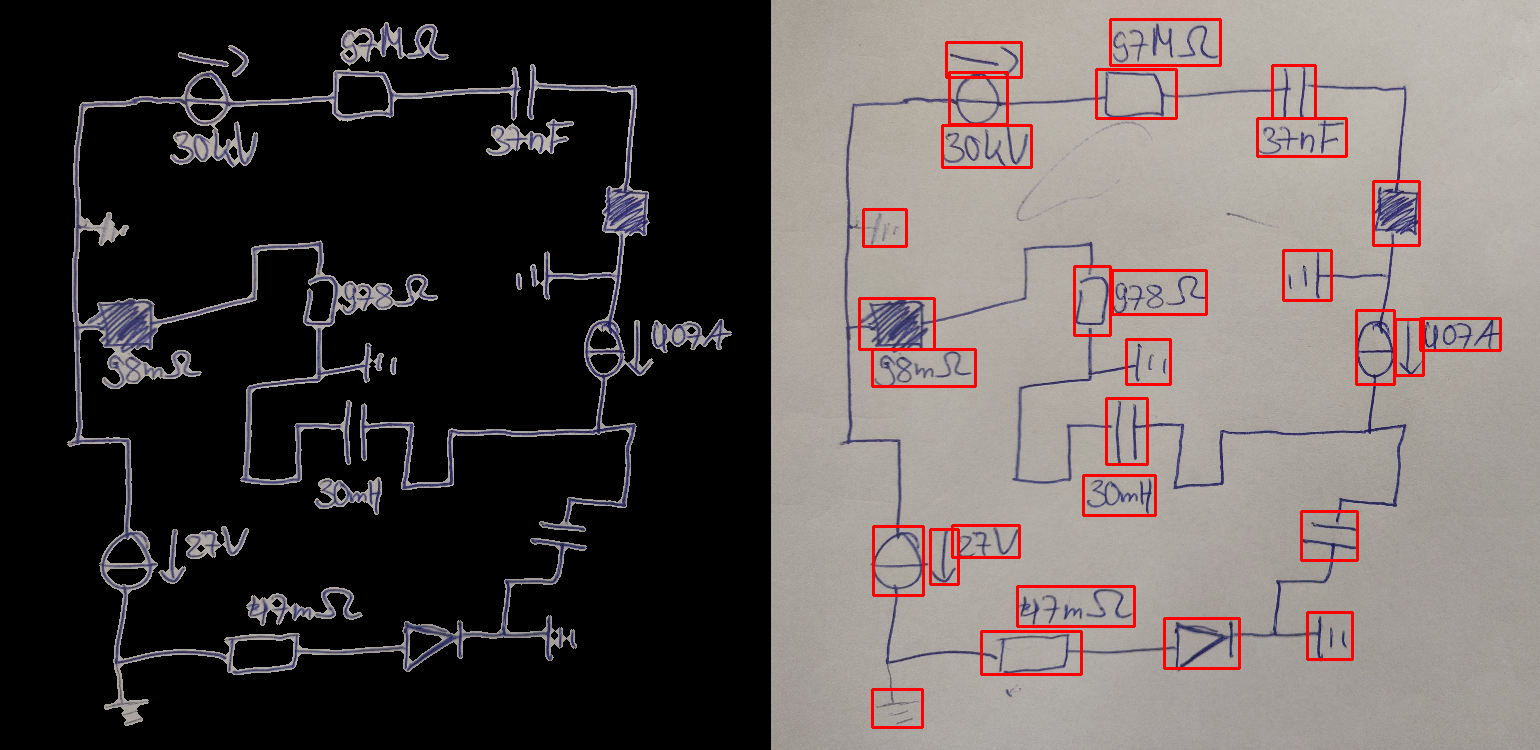
\includegraphics[width=\columnwidth]{imgs/labels/both_example.png}
    \caption{Example segmentation label mask (left) and bounding boxes labels (right).}
    \label{fig:example_labels}

\end{center}
\end{figure}

\begin{table}
\begin{center}
\begin{tabular}{l|l|l|l|l|}

\textbf{class} & \textbf{total} & \textbf{train ratio} & \textbf{valid ratio} & \textbf{test ratio} \\
    \hline
    diode left              & 156    &  83.33\%  &    8.97\%  &  7.69\% \\
    diode top               & 210    &  82.38\%  &    6.19\%  & 11.43\% \\
    diode right             & 150    &  82.00\%  &   12.67\%  &  5.33\% \\
    diode bottom            & 102    &  67.65\%  &   15.69\%  & 16.67\% \\
    resistor horizontal     & 318    &  71.38\%  &    6.92\%  & 21.70\% \\
    resistor vertical       & 350    &  66.00\%  &    6.57\%  & 27.43\% \\
    capacitor horizontal    & 405    &  85.68\%  &    4.94\%  &  9.38\% \\
    capacitor vertical      & 268    &  65.30\%  &   10.45\%  & 24.25\% \\
    ground left             & 137    &  72.99\%  &   10.95\%  & 16.06\% \\
    ground top              & 137    &  81.02\%  &   13.87\%  &  5.11\% \\
    ground right            & 116    &  78.45\%  &   14.66\%  &  6.90\% \\
    ground bottom           & 178    &  73.60\%  &   14.04\%  & 12.36\% \\
    inductor horizontal     & 251    &  76.89\%  &    8.37\%  & 14.74\% \\
    inductor vertical       & 290    &  73.45\%  &    9.31\%  & 17.24\% \\
    source horizontal       & 188    &  77.66\%  &   11.17\%  & 11.17\% \\
    source vertical         & 238    &  64.71\%  &   14.29\%  & 21.01\% \\
    current horizontal      & 202    &  77.72\%  &    9.41\%  & 12.87\% \\
    current vertical        & 220    &  75.00\%  &   12.73\%  & 12.27\% \\
    text                    & 877    &  61.92\%  &   16.76\%  & 21.32\% \\
    arrow left              & 57     &  70.18\%  &   19.30\%  & 10.53\% \\
    arrow top               & 77     &  64.94\%  &   23.38\%  & 11.69\% \\
    arrow right             & 105    &  70.48\%  &   16.19\%  & 13.33\% \\
    arrow bot               & 104    &  71.15\%  &   15.38\%  & 13.46\% \\
    \hline
    \textbf{total}          & 5136   &  73.65\%  &   12.27\%  & 14.08\% \\
\end{tabular}
\caption{The classes present in this thesis with their major class which is an \ac{ECC} and alternatively their orientation. Furthermore, the total amount of classes is shown and the train, valid, test ratio.}
\label{tab:yolo_classes}
\end{center}
\end{table}

\subsubsection{Labels: Topology}
\label{sec:hypergraph_topology}

The pipeline of this thesis produces a topology representing the underlying connections between \acp{ECC}.
To quantify the amount of errors in a produced topology (prediction), a ground truth is needed, against which the prediction is compared to.
The chosen prediction and ground truth format is an adjacency matrix of a hypergraph.
The labeling process as well as the evaluation with proposed algorithm is time consuming, therefore only the test dataset was labeled and evaluated in this thesis.
Especially due to the fact that the underlying problem, which the evaluation algorithm tries to solve, is NP-hard.
More details are explained in section \ref{sec:eval_algo}.
Following the label format of the \acp{ECD} is explained.

First a copy of the original \ac{ECD} was created, which was then populated with numbers above each component, which was labeled with a bounding box.
The number above each component corresponds to the index of that bounding box in the YOLO label file.
Those images were used as a visual helper in the topology labeling process.
An example of such an image can be found in figure \ref{fig:example_topology_label}.

\begin{figure}
\begin{center}

    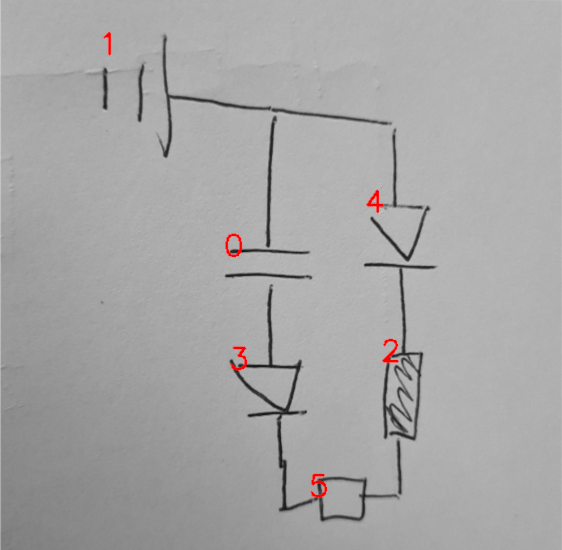
\includegraphics[width=11.1cm]{imgs/topology_label_idx_example.png}
    \vspace{2cm}

    \begin{tabular}{|l||l|l|l|l|l|l|l|l|l|l|l|l||l|}

    \hline
	\textbf{Index}  & 0 &   & 1 &   & 2 &   & 3 &   & 4 &   & 5 &   & \\
    \hline\hline
	\textbf{Edge 0} & 1 & 0 & 0 & 1 & 0 & 0 & 0 & 0 & 1 & 0 & 0 & 0 & 1r,0t,4t \\
    \hline
    \textbf{Edge 1} & 0 & 1 & 0 & 0 & 0 & 0 & 1 & 0 & 0 & 0 & 0 & 0 & 0b,3t    \\
    \hline
    \textbf{Edge 2} & 0 & 0 & 0 & 0 & 0 & 0 & 0 & 1 & 0 & 0 & 1 & 0 & 3b,5l    \\
    \hline
    \textbf{Edge 3} & 0 & 0 & 0 & 0 & 0 & 1 & 0 & 0 & 0 & 0 & 0 & 1 & 5r,2b    \\
    \hline
    \textbf{Edge 4} & 0 & 0 & 0 & 0 & 1 & 0 & 0 & 0 & 0 & 1 & 0 & 0 & 4b,2t    \\
    \hline

    \end{tabular}

    \caption{An example visual labeling helper image (top), shown with the index of the respective bounding box in the YOLO label file, together with the corresponding hypergraph adjacency matrix (bottom). Two columns in the matrix correspond to one \ac{ECC}, each column to one orientation, where the first column can either be the left or top orientation and the second column be the right or bottom orientation. The last column in the table further shows the string representation of an edge, which acts as the input for the labeling tool. For instance ``1r,0t,4t'' means that 1 right, 0 top and 4 top are connected to each other through a hyperedge.}
    \label{fig:example_topology_label}

\end{center}
\end{figure}

To now label the topology, first each index is split into to sub-indexes, each representing the orientation of the connection, where a connection is defined as the side where the wire is connected to.
For instance in figure \ref{fig:example_topology_label}, index 1 is a ground symbol and its connection is on the right side.
For index 0, which is a capacitor the connection is at the top and the bottom.
The two orientation pairs \{left, top\} and \{right, bottom\} are fused together into one column of the hypergraph adjacency matrix.
Given a hypergraph matrix, the orientation of a particular bounding box index n can be obtained with the index 2n or 2n+1, for the \{left, top\} or \{right, bottom\} orientation, respectively.
A connection, where multiple \acp{ECC} are connected is represented as a row in the adjacency matrix.
Figure \ref{fig:example_topology_label} shows how the hypergraph adjacency can be created from a visual helper image.

For the topology labeling a small labeling tool was created, where the algorithm should be shortly presented:

\begin{enumerate}
    \item Initialize a matrix of zeros with the size $N \times N$, where $N$ is the number of bounding boxes in the \ac{ECD}.
    \item Read user input in the form: ``\{Index$_x$\}\{Orientation$_x$\},...,\{Index$_y$\}\{Orientation$_y$\}'', where Index$_n$ represents the index of a bounding box and orientation $\in$ \{t, l, r, b\} (top, left, right, bottom),  which represents a complete edge in the hypergraph adjacency matrix. Do this until all edges have been entered.
    \item Store the produced hypergraph adjacency matrix.
\end{enumerate}


\subsubsection{Labels: Textual Annotations and Arrow Annotations}

In general all annotation types used in this work belong to an \ac{ECC} and therefore act as an extension of an \ac{ECC}.
Therefore, matching of annotations to their respective \ac{ECC} is part of this work and is presented in section \ref{sec:pipeline}.
To quantify the matching performance, a representation of the ground truth is needed.
The chosen label format builds on the visual helper image, presented in the topology labeling process.
A map is created, where the index of an \ac{ECC} is mapped against the index of the corresponding annotation.
Since, two different types of annotations are present, each annotation type receives an own label file.
A label file is created in the \ac{CSV} file format, where each line represents a matching pair of \ac{ECC} index and annotation index.
Hence, one file contains all matching pairs for textual annotations and the second one all matching pairs for arrow annotations.
